\documentclass[../main.tex]{subfiles}

\begin{document}

\onehalfspacing

En este capítulo, se explican los resultados de cada uno de los modelos de redes presentados en el capítulo de metodología.


El análisis se enfoca en dos perspectivas: i) se analizaron las redes $NC(h)$ y se calcularon sus métricas (sección de métricas del capítulo 2); y ii), en la red de pre-explosividad $\G{h}$, se realizó un análisis en las comunidades obtenidas y cómo favorecieron el comportamiento explosivo.

En esta sección solamente se presentan los principales resultados obtenidos en la investigación. Para un análisis más detallado, véaso el Anexo A.


\section{Análisis preliminar de las tendencias.}

La cantidad de usuarios partícipes es diferente en las tendencias con comportamiento explosivo de las tendencias sin comportamiento explosivo.  En las tablas del comparativo \ref{tab:comparativo_tendenciasnumerosdetweets}, al tener una mayor cantidad de usuarios es esperable obtener una mayor cantidad de tweets; sin embargo, el hecho de tener una gran audiencia no es suficiente para caracterizar las tendencias por su propiedad de explosividad.  De los datos, la figura \ref{fig:resultados_comparativotweetsusuarios} no muestra un diferenciador para las tendencias con comportamiento explosivo. 

\begin{table}[!h]
    \centering
    \caption{Comparativo entre las tendencias por el número de usuarios totales que interactuaron en ella. En la tabla de la izquierda corresponden a tendencias con comportamiento explosivo (\textbf{CE}); del lado izquierdo aquellas sin comportamiento explosivo (\textbf{sCE}).}
    \label{tab:comparativo_tendenciasnumerosdetweets}
    \begin{tabular}{cc}
    \begin{minipage}{.5\linewidth}
        \begin{tabular}{ll}
            \toprule
                 Tendencias CE  &  No. de usuarios  \\
\midrule
        \textit{wheniwaslittle} &        20,150  \\
   \textit{yougetmajorpointsif} &        15,219  \\
            \textit{top100lies} &        13,129  \\
 \textit{nationalbestfriendday} &        12,569  \\
\textit{mythoughtsduringschool} &        10,662  \\
\bottomrule
        \end{tabular}
    \end{minipage} &

    \begin{minipage}{.5\linewidth}
        \begin{tabular}{ll}
            \toprule
 Tendencia sCE &  No. de usuarios  \\
\midrule
   \textit{fml} &         9,467 \\
   \textit{wtf} &         8,467 \\
  \textit{fail} &         7,283 \\
  \textit{2omf} &         6,957 \\
\textit{ohwell} &         6,915 \\
\bottomrule
        \end{tabular}
    \end{minipage} 
\end{tabular}
\end{table}

\begin{figure}[h!]
    \centering
    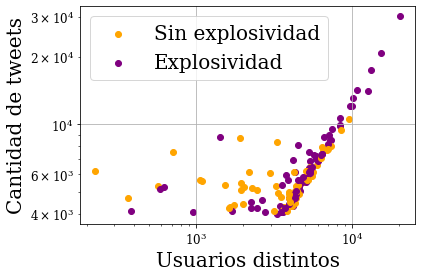
\includegraphics[scale = 0.8]{images/resultados_estadisticos.png}
    \caption{Comparativo de tendencias por la cantidad de usuarios registrados respecto a la cantidad de tweets recabados. }
    \label{fig:resultados_comparativotweetsusuarios}
\end{figure}

\section{Análisis de Comunidades.}

En esta sección, se analizarán dos momentos importantes de la interacción de los usuarios por cada tendencia a través del tiempo: Minutos previos a la mayor interacción en la red social $\G{h}$ y el momento de la mayor interacción en la red $NC_{t^{*}}(h)$. 

% Además, la red $\G{h}$ sobre los periodos de 25 a 50 minutos antes del periodo $t^{*}$ como se mencionó con más detalle en la sección de metodología.

Cabe recalcar que la principal diferencia entre las redes $\G{h}$ y $NC^{T}_{t^{*}}(h)$ es la escala y el tiempo de análisis. Es decir, al analizar la red $NC^{T}_{t^{*}}(h)$ interesa la dinámica del comportamiento explosivo en el momento del pico de interacción ($t^{*}$). En cambio, de la red $\G{h}$ interesa conocer más sobre la estructura de la red social que llevó al comportamiento explosivo. Considerar esta diferencia permite analizar los resultados desde una perspectiva cualitativa y desde un enfoque predictivo.


\subsection{Comunidades con comportamiento similar.}

%En la primera parte (esta también puede ser opción) 
El primer paso fue determinar  el grado de asortatividad $(r)$ de la red $NC_{t^{*}}^{T}(h)$. Dicha métrica denota distribuciones de grado heterogéneas cuando el valor es negativo; es decir, hay nodos de grado alto enlazados con nodos de grado bajo indicando que la red es disortativa. Además, se puede denotar la existencia de enlaces puente cuando $r$ es negativo. 

En los resultados, un menor grado de disortatividad de las redes $NC_{t^{*}}^{T}(h)$ etiquetadas por la propiedad de explosividad, resulta ser significativa (95\% de confianza por Kolmogorov-Smirnov). Es decir, la red social de los comunicantes de tendencias con comportamiento explosivo resultan ser menos disortativas. Esta diferencia es visible en la figura \ref{fig:results_RmaxInteract}. 


\begin{figure}[h!]
    \centering
    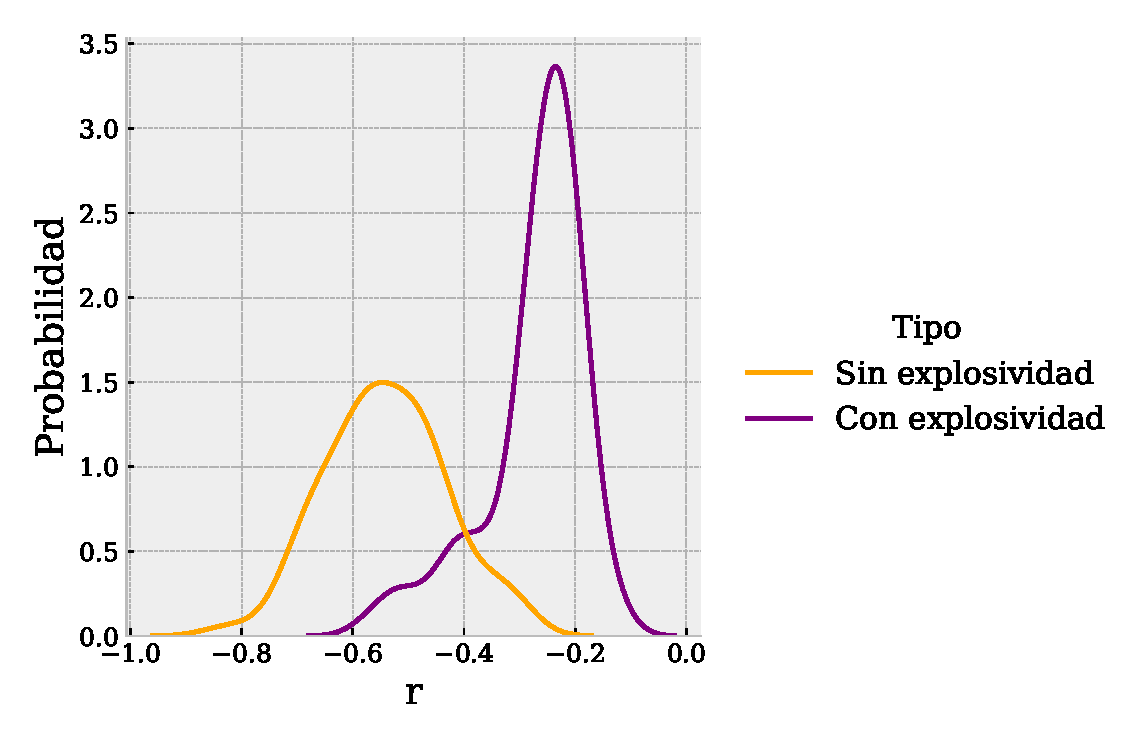
\includegraphics[scale = 0.7]{images/results_Rmaxinteract.pdf}
    \caption{Histograma de la asortatividad de las redes por su tipo de comportamiento. La diferencia en medias es significativa.  }
    \label{fig:results_RmaxInteract}
\end{figure}

%Aquí usamos $\G{h}$
Por otro lado, una mayor cantidad de comunidades partícipes marca la diferencia de tendencias con comportamiento explosivo de las que  lo son (95\% de confianza por Kolmogorov-Smirnov). En la tabla \ref{tab:resulatdos_comparativodecomunidades}, se aprecia como la media del número de comunidades es mayor en tendencias con comportamiento explosivo. Este resultado se puede visualizar de la figura \ref{fig:resultados_lenComunidades}. % donde se  muestra como las tendencias con comportamiento explosivo deben tener un mayor número de comunidades interactuando. 




% ---OPCIONES----
% Comparativo de estadíaticos el número de comunidades. 
% Comparativo de la s estd de la com xonsiderando explo y sin explo
% 
% Estadísticas de  comunidades considerando explosividad.

%MOSTAR QUE ES LO Q

%Una opción, puede que 
\begin{table}[]
    \centering
    \caption{Comparativo de las estadísticas de la cantidad de comunidades considerando la propiedad explosividad y sin explosividad.}
    \label{tab:resulatdos_comparativodecomunidades}
    \begin{tabular}{lrr}
\toprule
{} &  Explosividad &  Sin explosividad \\
\midrule
Promedio de la cantidad de comunidades  &    167.951807 &         99.416667 \\
Menor cantidad de  comunidades  &      8.000000 &          6.000000 \\
Máxima cantidad de comunidades   &    363.000000 &        418.000000 \\
\bottomrule
\end{tabular}
\end{table}




\begin{figure}
    \centering
    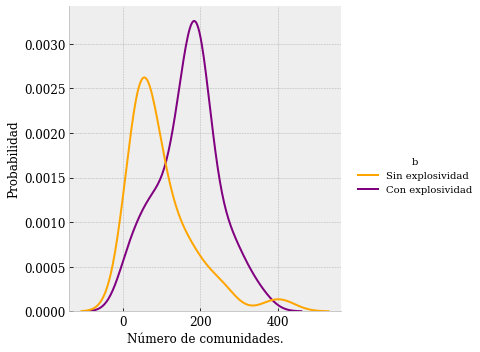
\includegraphics[scale = 0.6]{images/resultados_comparativocomunidades.png}
    \caption{Histograma del número de comunidades de las redes $\G{h}$ por su tipo de comportamiento. Se observa la existencia de un sesgo significativo que caracteriza a las tendencias.}
    \label{fig:resultados_lenComunidades}
\end{figure}


\newpage
\subsection{Incremento de comunidades  respecto al tiempo}
% -------------------------------
% NO ES JUSTIFIACIÓN, ES EXPLICACIÓN DE LOS RESLULTADOS EN FUNCIÓN DEL PROCEDIMIENTO
% TODO VERLOS DE MANAREA RESTROSPECTIVA (SOLO VER LO QUE PASÓ) 
% -------------------------------
%Nota: No sé si estoy hablando de comunidades. 
% De lo que hablo es la parte del kcore

\begin{figure}[h!]
    \centering
    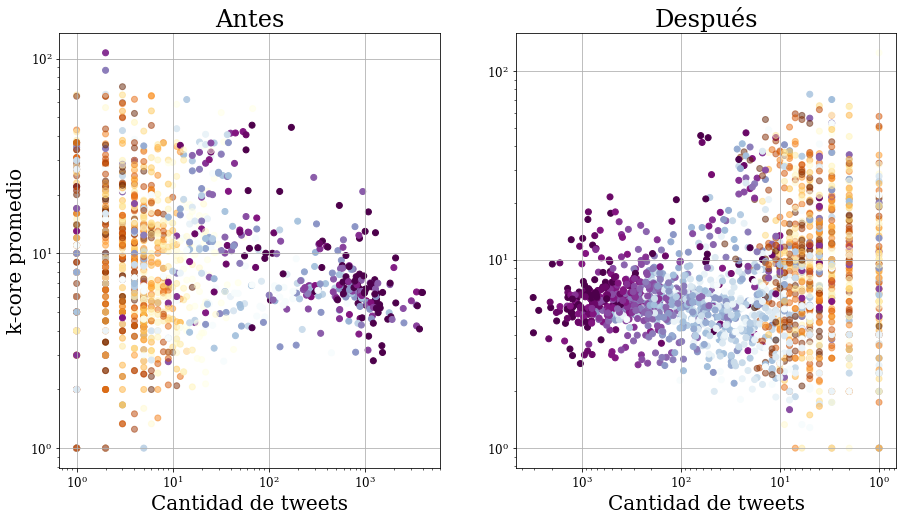
\includegraphics[scale = 0.37]{images/resultados_peakKcore.png}
    \caption{Comparativo del $k-core$ de los usuarios partícipes antes y después del momento de mayor interacción (\textbf{peak}). De color rojo son aquellas tendencias con comportamiento explosivo. }
    \label{fig:resultados_kcoregrafico}
\end{figure}

%Marcar un diferenciador entre las minisecciones, 

Un paso relevante fue el cálculo del \textit{k-core} en las redes $\G{h}$. Este cálculo permite identificar qué tan lejanos están los nodos que publicaron un tweet, respecto al centro de su comunidad. Es decir, se espera encontrar una capa en la comunidad donde se realice la mayoría de las  interacciones. 


Los resultados se obtuvieron con el siguiente procedimiento. De la red $\G{h}$, se generó el valor k-core para cada nodo. Después, se identificaron aquellos nodos que realizaron algún \textit{tweet}. Así, para generar una sucesión de números, se agruparon los nodos en intervalos de tiempo de 15 minutos antes y después del momento de mayor explosividad. Finalmente, se obtiene la media de los valores recolectados por cada intervalo de tiempo. En la figura \ref{fig:resultados_kcoregrafico}, se aprecian dos gráficas de los resultados obtenidos en este proceso. 



% El comportamiento de las tendencias con propiedad de explosividad 
La interpretación de los resultados indica una capa donde se caracteriza la interacción relevante. Es decir, hay un valor del valor k-core que distingue las tendencias de comportamiento explosivo de las que no son. 

Antes de la mayor interacción, el k-core, no tiene un valor establecido para las tendencias. Sin embargo, en el último intervalo de tiempo antes de la mayor interacción, el valor k-core de los nodos es cercano a 10.

Después de la mayor interacción, el valor k-core se dispersa con una tendencia a la disminución. En otras palabras, la interacción ya no es gobernada por nodos donde su k-core es cercano a 10.


% Esto indica, que las tendencias con comportamiento explosivo no ocurre en una capa lejana o cercana al centro de cada comunidad; pero induce una interacción con el centro de cada comunidad y, posteriormente, se esparza la información en sus capas más lejanas. 



% Lo que se observa en los resultados es .... :c





%¿Cómo\textit{ }puedo concluir esto? 
%Cómo fomalizar esra diferencia? 





\section{Análisis Global de la Dinámica de las Tendencias.}


En esta sección, se explicará con detalle el cálculo que se realizó para la red $NC_{t}^{T}(h)$ por cada tendencia $h$. Cabe recordar que la red $NC(h)$ es una red temporal multicapa, en este caso (ver la sección de metodología),  $NC^{T}(h)$ es una red no dirigida y $NC_{t}^{R}(h)$ es una red dirigida donde $t$ es un periodo de tiempo fijo. Cada una en estas redes representa a un usuario que participó con algún tweet o retweet en el periodo de tiempo $t$.

Con esto en mente, es factible aplicar diversas métricas conocidas de redes. Por ejemplo, para la red $NC_{t}^{T}(h)$ se puede calcular el coeficiente de asortatividad y para $NC_{t}^{R}$ se puede obtener la media del grado exterior. 



Con esto en mente, se realizaron los siguientes cálculos, especificando en qué red fue aplicada.  

\begin{itemize}
    \item Para cada $NC_{t}^{T}$ donde $t$ es una ventana de tiempo.  
    \begin{enumerate}
        \item Grado promedio.
        \item Media del camino más corto. 
        \item Cálculo del coeficiente de centralidad clustering
        \item Cálculo del coeficiente de centralidad betweenness %Esta no pasa KruskalWallis
        \item Cálculo de la entropía de Shannon de la distribución de grado. 
        \item Grado promedio 
    \end{enumerate}
    \item Para cada $NC_{t}^{R}$  
    \begin{enumerate}
        \item Grado exterior más grande. 
        \item Diámetro más grande. 
    \end{enumerate}
\end{itemize}

De cada tendencia se obtuvo una serie de tiempo por cada una de las métricas. Para inferir un valor característico en cada una de estas métricas, se procedió a calcular un estadístico en cada una de estas serie de tiempo. Por un lado, para las métricas relacionadas a la red no dirigida $(NC_{t}^{T})$ se obtuvo la media de cada una de las  series de tiempo. Por otro lado, para las redes dirigidas, se procedió a calcular el máximo valor de esta serie de tiempo. 

A partir del cálculo de estos estadísticos, se empiezan a notar diferencias entre las tendencias. Se puede notar de la tabla \ref{tab:resultados_diferenciasDeTendencias}, que la diferencia entre el comportamiento de tendencias resulta ser estadísticamente significativo a través de la prueba de Kruskal-Wallis %(95\% de confianza) (ver pruebas paramétricas en anexo X).
% También puede ser (en el anexo X se puede consultar las pruebas paramétricas) 

\begin{table}[h!]
    \centering
    \caption{Valores $p$ obtenidos al aplicar la prueba no paramétrica de Kruskal-Wallis. }
    \begin{tabular}{lr}
\toprule
      Estadística  &       \textit{$p-value$} \\
\midrule
     Media de la cantidad de Tweets por hora  &  $1.585502\text{x}10^{-16}$ \\
   Media de la cantidad de retweets &  $2.797278\text{x}10^{-18} $\\
    Media del grado promedio &  $5.785002\text{x}10^{-02}$ \\
    Media del promedio de longitud del camino más corto   &  $2.423004\text{x}10^{-20}$ \\
  Media del clustering &  $1.419858\text{x}10^{-07}$ \\
 Media del betweenness &  $2.560294\text{x}10^{-01}$ \\
     Media de la entropía &  $2.288698\text{x} 10^{-18}$ \\
     Diámetro más grande &  $4.843335\text{x} 10^{-14}$ \\
        Vecindad más grande &  $1.283606\text{x} 10^{-15}$ \\
\bottomrule
\end{tabular}
    \label{tab:resultados_diferenciasDeTendencias}
\end{table}


% \section{ Valores significativos en la entropía, clustering y betweenness. }
\subsection{ Valores Significativos en la Dinámica Total y en el Pico de Interacción.  }


 

% La distribución de grado de una red provee un primer acercamiento a la investigación de la red en cuestión. Al considerar la distribución de grado como una probabilidad, permite el uso de diversas herramientas probabilísticas como la  entropía de Shannon. El estudio de esta métrica aplicada en redes ha sido corto y en casos muy particulares: En el caso de redes de acitvida neuronal, la entropía de Shannon fue útil para no descartar la teoría entrópica del cerebro  \cite{ayahuasca_Viol2017} o, en un hiperplano meramente matemático, se concluyó que la entropía de la distribución de grado es una medida efectiva de la resiliencia de la red en ataques aleatorios \cite{entropia_opti}. En ambos artículos, se destaca un uso de la entropía de Shannon en la distribución de grado para destacar a la red diferencias no obvias de redes. 
% Con el desarrollo de las seccionesa ant, se procede al desarrollo y análisis de los resultados. 

\begin{figure}[h!]
    \centering
    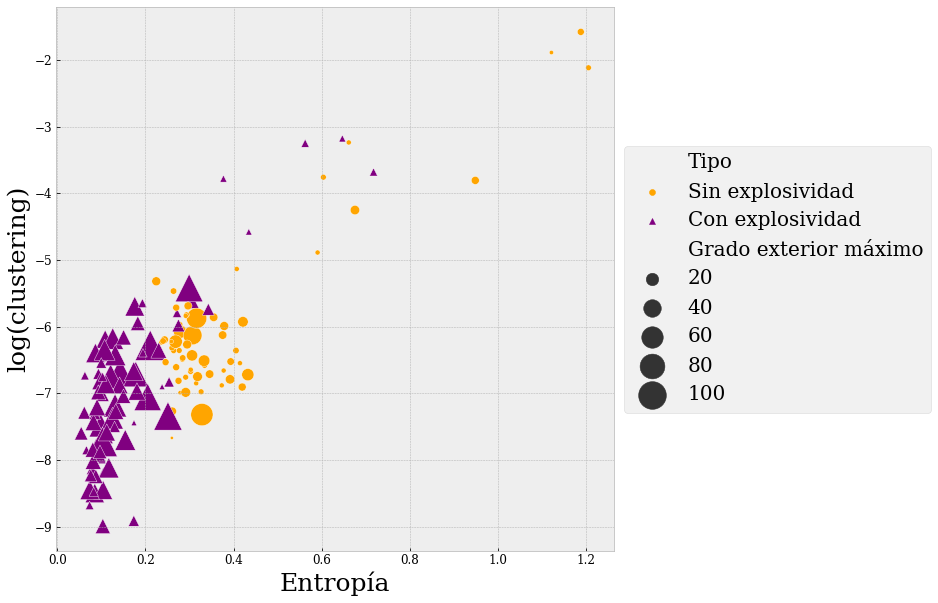
\includegraphics[scale = 0.40]{images/results_entropyVSclustering.png}
    \caption{Comparativo entre las tendencias respecto a las métricas calculadas. El tamaño de cada uno de los marcadores es proporcional al máximo del grado exterior máximo de cada una de las tendencias. }
    \label{fig:results_entropyVSclustering}
\end{figure}

La entropía de Shannon (\ref{shannon-entropy}) es una medida de incertidumbre para una variable aleatoria. Por su propia construcción, es positiva  y  no se enfoca en los valores de la variable aleatoria; se da énfasis en la probabilidad de los eventos más no el evento en sí. Se especifica en la incertidumbre del estado actual. 

%valor correspondiente de
En las figuras \ref{fig:results_entropyVSclustering} y \ref{fig:results_entropyVSbetweeness}, se observa la relación entre el comportamiento explosivo y la  entropía. Si bien algunos datos son atípicos, las tendencias con comportamiento no explosivo tuvieron un valor mínimo en la entropía (0.25 aprox.). Con base en la entropía de Shannon, la red de las tendencias con comportamiento explosivo son homogéneas en la distribución de grado. 

\begin{figure}[h!]
    \centering
    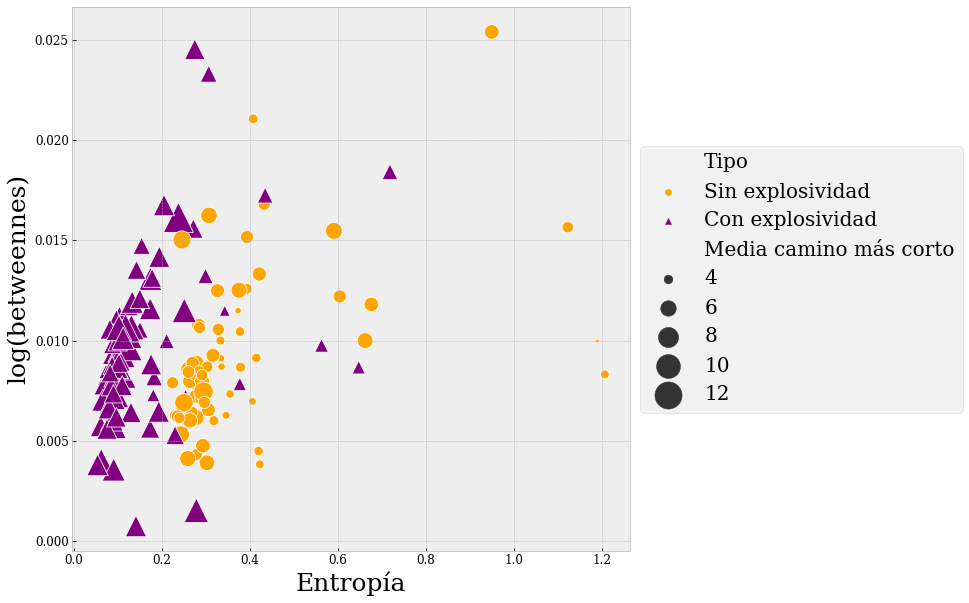
\includegraphics[scale = 0.40]{images/results_entropyVSbetweennes.png}
    \caption{Comparativo de tendencias entre   betweenness (media) y entropía. El tamaño de cada uno de los marcadores del gráfico está en proporción de la media del camino más corto. }
    \label{fig:results_entropyVSbetweeness}
\end{figure}

% Comparativo de tendencias a través de la media de las métricas betweenness y entropia. El tamaño de cada uno de los marcadores del gráfico está en proporción de la media del camino más corto.

También se obtuvieron relaciones interesantes entre las métricas betweenness y entropía. En la figura \ref{fig:results_entropyVSclustering},  se observa una  correlación lineal positiva entre entropía y clustering. Una correlación esperable ya que al incrementar el clustering, se incrementa el número de triángulos y, por tanto, se incrementa el grado de los nodos.  Además, en la misma figura, se puede apreciar como el beneficio de actividades de costo mínimo, como los retweets, propician que la tendencia sea de comportamiento explosivo. Esto último puede ser consecuencia del tipo de tendencia. 

% Esto último puede ser consecuencia del tipo de tendencia o tema que se requiera discutir

% Esto último puede ser consecuencia del tipo de tendencia; del artículo \cite{REDDIT} nos dan un pequeño análisis de comunidades sobre \textit{subreddits} (comunidades más pequeñas) mostrando que aquellas con pocas personas pero con una organización clave entre las demás, pueden generar enfrentamientos masivos; misma idea fue hecha \cite{Conover_Ratkiewicz_Francisco_Goncalves_Menczer_Flammini_2011}, sobre discusiones políticas en \textit{Twitter}. Lo cual, al considerar la poca incertidumbre de la entropía de Shannon, es consistente con la bibliografía de comunidades pequeñas pero organizadas. 

En resumen, se necesita cierta homogeneidad entre comunidades para generar el comportamiento explosivo. Específicamente, que esa homogeneidad no rebase una entropía de 0.25. Por otro lado, también debe existir la necesidad de acciones de menor costo y con tiempos específicos. La dinámica de \textit{Twitter} es una comunicación sencilla y simple, y la acción de \textit{retweet} es la que recapitula la mayor cantidad de interacciones.   


%TODO: CHECAR ESTA SECCIÓN

% \subsection{ Actividad conjunta de comunidades } % y.   }

% %---------------------------------------
% %---------------------------------------
% %LOS HORARIOOOOOOOOOOOOOOOOOOOOOOOOOOOOS
% %---------------------------------------
% %---------------------------------------

% El análisis de complejidad casi siempre consiste en encontrar patrones recurrentes en las configuraciones siempre cambiantes del sistema. En ese sentido, el estudio de comunidades permite la identificación de patrones.




% Algunos datos y conclusiones que quiero y estoy obteniendo. 

% % - Sí hay una diferencia marcada entre las tendencias por el número de comunidades que participan. Se puede ver de la tabla \ref{tab:resulatdos_comparativodecomunidades}



% %PArece que hay una relación. 
% %Mencionarlo pero nunca concluirlo. Se necesitarían más pruebas. 
% %Con el trabajo realizacdo, no es posible conclkuir si un caso favorece al otro. 
% % ES decir, si mayor cantidad de tweets genera mayor comunidades (o viceversa) 
% % Nada de conclusión. !!!!!!!!!!!!!!!!!!!!!!!!!!

% % Polarización??? Ponerlo como nota extra y me lavo las manos :D 

% %Ni +Tweets !=> +Comunidades



% % No se generan enlaces fuertes. Son ences débiles. 

% % Estas ideas extras, si no salen, se quedan en trabajo futuro. 

%     - De esta tabla, tenemos sobre toda la dinámica. 
    
% - Si bien son muchas comunidades, esto no nos dice nada de ellas. 

% Qué podemos decir del tiempo? 
%     - El gráfico cuando hacemos con el tiempo sí nos marca que cierta repetición 

%     - Del core, tenemos que es pequeño. Es decir, tal vez sean comunidades pequeñas pero muchas (de esto el primer artículo es el que nos acompaña con esta El gráfico)  (Esto puede ir en discusión)
%     % Comunidades peque!nas por el k core. \

    
%     % Se abren a más comunidades -> Crecen conforme van apareciendo los tweets.
    
%     % PEnsar de otra forma la parte del 
%     % Del tiempo, sería mostrar mejor los timepos y la fórmula. 
    
%     % DISCUSIÓN DE LO DE AQU;I
%     - De la entropía, nos dice que su distribución de grado no es aleatoria. Es decir, las comunidades son pequeñas y con un comportamiento más esperable (es decir homogéneas) (Esto igual)
%     % Va para arriba. 
    
%     %Comunidades crecen -> Comunidades peque!nas
    
%     % Hacer la pruebita con la fórmula de Miritello (PERO PRUEBITA) 
    
    
    


% % Esto va a comunidades. 
% % - Hasta ahora, 
% %     Comunidades de las redes asociadas a tendencias de comportamiendo explosivo. 
% %         - Muchas
% %         - Pequeñas
% %         - Son menos agrupadas. 
% %         - La distribución de grado puede ser esperable (por la entropía). 



% % Hay diferencias entre comunidades. 
% % Se podría concluir que 
% %costo menor
% %costo bajo
% %costo mínimo

\end{document}

% Se reacciona al comportamiento de las personas maas no de la gente.


\begin{figure}
    \centering
    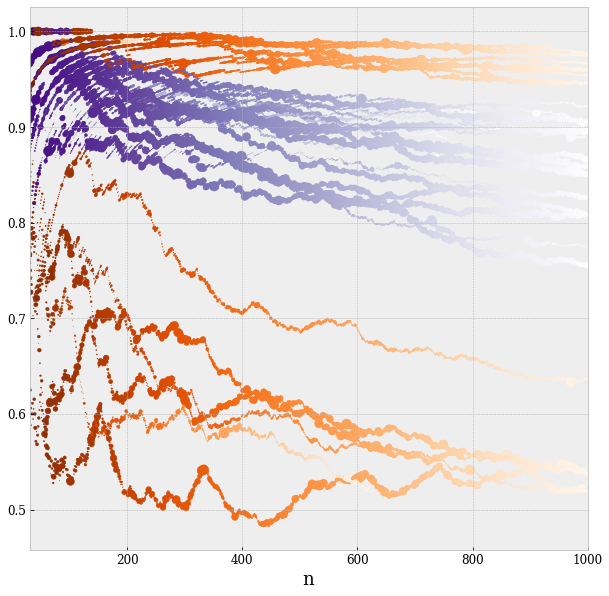
\includegraphics[scale = 0.5]{images/resultados_razonusuarios.png}
    \caption{ Comparativo de tendencias por los primeros 1000 \textit{Tweets}. Razón de usuarios nuevos en cada \textit{tweet} de los 1000 \textit{tweets} antes del periodo $t^{*}$. La líneas de color morado corresponden a tendencias con comportamiento explosivo.  } 
    \label{fig:resultados_1000Tweets}
\end{figure}